
    
    \chapter{Grayscale}

    \section{Performance Tests}

    \begin{center}
        \begin{figure}[H]
            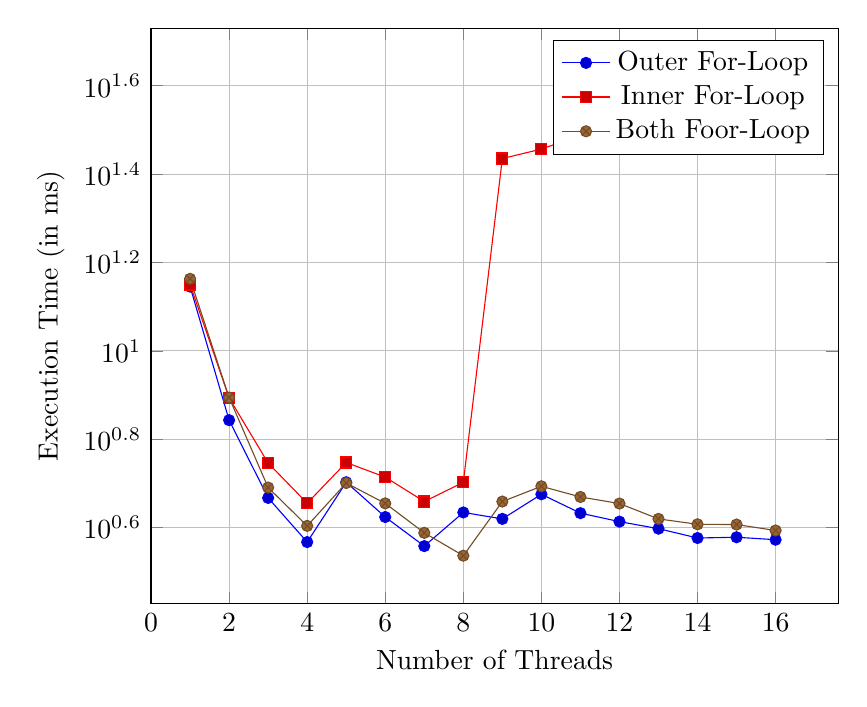
\begin{tikzpicture}
                \begin{axis}[
                    title={},
                    width=0.85\textwidth,
                    xlabel={Number of Threads},
                    ylabel={Execution Time (in ms)},
                    xmin=0,
                    ymin=0,
                    ymode=log,
                    grid=major
                ]
                    \addplot coordinates {
                        (1,13.9745)(2,6.96595)(3,4.6442)(4,3.68995)(5,5.03995)(6,4.20395)(7,3.61295)(8,4.3057)(9,4.1637)(10,4.7335)(11,4.28995)(12,4.10465)(13,3.9569)(14,3.76905)(15,3.7839)(16,3.7353)
                    };
                    \addlegendentry{Outer For-Loop}

                    \addplot coordinates {
                        (1,14.1323)(2,7.823)(3,5.5688)(4,4.5187)(5,5.58615)(6,5.1761)(7,4.5574)(8,5.0374)(9,27.2378)(10,28.6125)(11,30.7489)(12,33.5384)(13,35.3871)(14,36.3363)(15,39.2266)(16,41.8422)
                    };
                    \addlegendentry{Inner For-Loop}       

                    \addplot coordinates {
                        (1,14.5495)(2,7.8367)(3,4.9025)(4,4.01435)(5,5.0195)(6,4.5141)(7,3.8719)(8,3.4367)(9,4.55745)(10,4.93435)(11,4.66755)(12,4.50995)(13,4.16325)(14,4.048)(15,4.0425)(16,3.9195)
                    };
                    \addlegendentry{Both Foor-Loop}
                \end{axis}
            \end{tikzpicture}
            \caption{Grayscale Performance Tests}
        \end{figure}
    \end{center}


    \section{Implementation}

    

    \begin{listing}[H]
        \begin{minted}{cpp}
cv::Mat applyGrayscaleOuter(cv::Mat srcImage, int numThreads = omp_get_num_procs()) {
    auto destImage = cv::Mat(srcImage.rows, srcImage.cols, CV_8UC1);

    omp_set_num_threads(numThreads);

    #pragma omp parallel for default(none) shared(srcImage, destImage)
    for (int row = 0; row < srcImage.rows; row++) {
        for (int col = 0; col < srcImage.cols; col++) {
            auto srcPixel = srcImage.at<cv::Vec3b>(row, col);

            uchar r = srcPixel[2];
            uchar g = srcPixel[1];
            uchar b = srcPixel[0];

            // uchar destPixel = 0.21 * r + 0.72 * g + 0.07 * b; // luminosity formular
            uchar destPixel = 0.299 * r + 0.587 * g + 0.114 * b; // open cv formular

            destImage.at<uchar>(row, col) = destPixel;
        }
    }

    return destImage;
}
        \end{minted}
        \captionof{lstlisting}{Grayscale with parallelization of the outer For-Loop}
        \label{listing:grayscale}
    \end{listing}


\section{Comparison with OpenCV}

\subsection{Code}

\begin{listing}[H]
    \begin{minted}{cpp}
cv::Mat applyOpenCvGrayscale(const cv::Mat &srcImage) {
    cv::Mat destImage;
    cv::cvtColor(srcImage, destImage, cv::COLOR_BGR2GRAY);

    return destImage;
}
    \end{minted}
    \captionof{lstlisting}{Grayscale with OpenCV}
    \label{listing:grayscale_opencv}
\end{listing}

\subsection{Performance}

